Para comenzar el proceso del desarrollo del traductor del que se habló en las secciones anteriores, decidimos basarnos en 3 (tres) modelos clásicos implementados en System Dynamics. Estos son: el modelo \textbf{Teacup} (modela una taza de café en una habitación, que se enfría progresivamente hasta alcanzar la temperatura ambiente), el modelo \textbf{SIR} (modela una población que sucumbe ante una infección que se propaga en la misma, y posteriormente se va recuperando, hasta que no queda ningún infectado), y el modelo \textbf{Lotka-Volterra} (modela el proceso de nacimientos y decesos de un población de linces y liebres, que interactúan entre sí con una dinámica de presa-depredador).

Mediante el estudio de estos tres problemas, analizamos cómo los diferentes elementos de cada archivo xmile pueden ser traducidos a elementos de un modelo acoplado DEVS (expresado en formato DEVSML), de forma tal que esta traducción, al ser ejecutada (en este caso en el simulador CD++), replique los resulados que se obtienen simulando el modelo original en simuladores se SD.

A continuación, exponemos cada uno de los modelos mencionados, mencionando cómo nos ayudaron en el desarrollo del traductor. Aprovecharemos que el modelo Teacup traducido contiene pocos archivos para mostrar el código generado, por el traductor, mientras que para la exposición del comportamiento de los otros modelos cuya traducción genera una mayor cantidad de archivos, utilizaremos el lenguage formal típico con que se expresan modelos DEVS.

\subsection{Modelo Teacup}
\subsubsection{Modelo gráfico}
Como se puede observar en la figura \ref{fig:Teacup_sd} se cuenta con 1 (un) stock, que llamamos \textit{Teacup Temperature}, 2 (dos) constantes auxiliares (\textit{Room Temperature} y \textit{Characteristic Time}) y un flujo de salida (outflow) denominado \textit{Heat Loss to Room} con origen el stock \textit{Teacup Temperature} y destino vacío. Las flechas negras indican que el flujo de salida proveniente de \textit{Teacup Temperature} utiliza dicha constantes auxiliares en su función interna para determinar el valor de dicho flujo de salida en cada instante en el tiempo. La flecha azul, indica que dicha función también utiliza el valor del stock \textit{Teacup Temperature} para hacer este cálculo. 
\begin{figure}[!h]
\centering
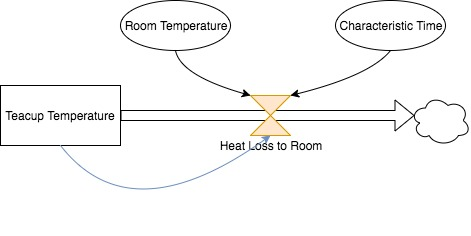
\includegraphics[scale=0.5]{imagenes/Teacup_sd.jpg}
\caption{Modelo Teacup expresado en System Dynamics en formato gráfico}
\label{fig:Teacup_sd}
\end{figure}

\begin{figure}[!h]
\centering
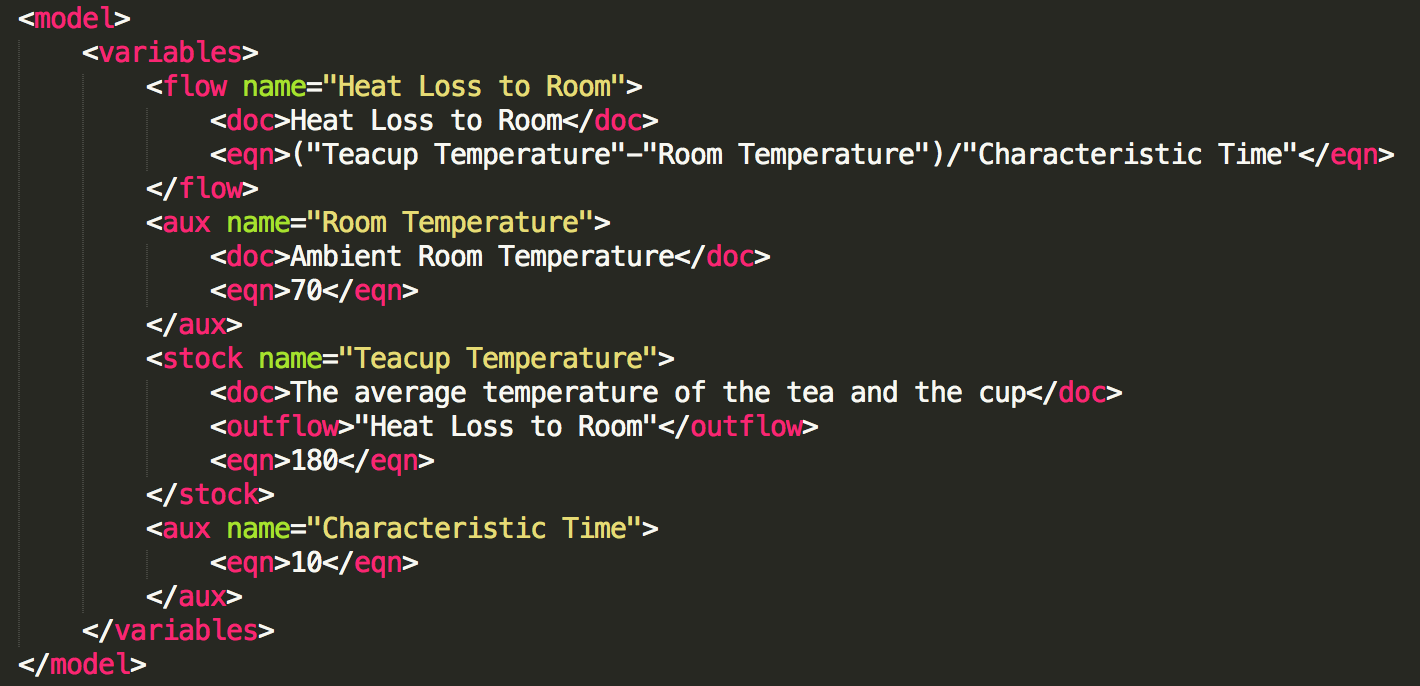
\includegraphics[scale=0.5]{imagenes/teacup_mapeo/Teacup_variables}
\caption{Modelo Teacup exprsado en System Dynamics en formato XMILE}
\label{fig:Teacup_xmile}
\end{figure}

Como se puede observar en la figura \ref{fig:Teacup_xmile}, se utilizan tres tags distintos para los flujos de output e inflow (el tag \textbf{flow}), para las constantes auxiliares (el tag \textbf{aux}) y para los stocks (el tag \textbf{stock}). Asimismo, en cada flujo, se utiliza un tag \textbf{eqn} para mostrar la función utilizada por dicho \textit{flow} (que puede ser tanto de input ó output) para agregarle o quitarle respectivamente unidades al stock sobre el cuál operan. Por otro lado, observamos que en los stocks y variables auxiliares se utiliza el tag \textbf{eqn} para mostrar el valor inicial de dicho stock ó variable auxiliar. Vale la pena aclarar aquí que en el caso de la variable auxiliar, esta podría ser tanto constante como variable. En este caso en particular, las variables auxiliares son todas constantes, con lo cuál en el tag \textbf{eqn} el valor inicial que figura en dicho tag también es el mismo valor que tendrá dicha variable durante toda la simulación. 

A partir de estas observaciones, decidimos representar este mismo modelo en el formalismo DEVS, de la forma en que se muestra en el diagrama de la figura \ref{fig:Teacup_devs_flattened}

\begin{figure}[!h]
\centering
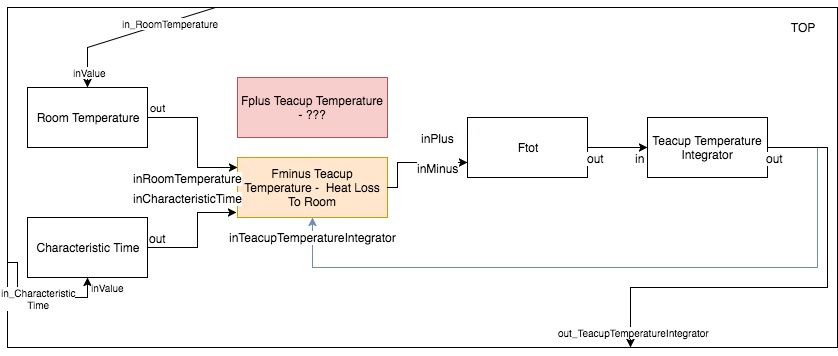
\includegraphics[scale=0.5]{imagenes/Teacup_devs_flattened}
\caption{Modelo Teacup expresado en DEVS en formato gráfico}
\label{fig:Teacup_devs_flattened}
\end{figure}

En el diagrama de la figura \ref{fig:Teacup_devs_flattened} se debe observar lo siguiente: a cada tag \textbf{stock} corresponden: 1 (un) atómico de nombre \textit{nombreStock + Integrator} y 1 (un) atómico Ftot, que acumula todos los inflows y outflows que operan sobre dicho stock para luego efectuar el cálculo final (que es una resta) entre los inflows y los outflows, para determinar la variación de unidades que tendrá dicho stock. 

Por otro lado, a cada flujo (en este caso \textit{Heat Loss to Room} corresponden: 1 (un) atómico de nombre \textit{Fminus + nombre del stock sobre el que opera restándole unidades + nombreFlujo}, cuyo output llega a la Ftot correspondiente al integrador sobre el que este opera restándole unidades; y 1 (un) atómico de nombre \textit{Fplus + nombre del stock sobre el que opera sumándole unidades + nombreFlujo}. En el ejemplo de la figura \ref{fig:Teacup_devs_flattened}, el flujo Fplus no tiene sentido ser, porque no hay ningún inflow que actúe sobre el stock \textit{Teacup Temperature}. Es por esto que lo marcamos en rojo para evidenciar que este stock no debería estar ahí porque no tiene ningún rol en el modelo. 

Finalmente, se observa que a cada tag \textbf{aux} hacemos corresponder un atómico DEVS cuya salida llega a los atómicos correspondiente al flujo \textit{Heat Loss to Room} que utilizan dichar variables para hacer sus cálculos. En este ejemplo, sólo se conectan con el \textit{FminusTeacupTemperature - Heat Loss to Room}, porque el stock \textit{Teacup Temperature} no tiene ningún inflow. 

También podemos observar en el diagrama la línea azul, que se corresponde con la línea azul del diagrama \ref{fig:Teacup_sd}. De esta forma, mostramos que el atómico \textit{FminusTeacupTemperature - Heat Loss to Room} utiliza también el output del atómico \textit{Teacup Temperature Integrator} para realizar sus cálculos. 

Llegados a esta instancia, nos preguntamos qué pasaría con nuestro mapeo a DEVS si más de un outflow operara sobre \textit{Teacup Temperature}. Así, decidimos pensar cómo sería la traducción gráfica del siguiente modelo (figura \ref{fig:Teacup_sd_2}), que modela un segundo outflow que opera sobre el stock \textit{Teacup Temperature} (en el ejemplo, decimos que la taza no sólo se enfría de acuerdo al rate de pérdida de calor de la taza contra la habitación, sino también contra una máquina enfriadora \textit{Cooling Machine} que agregamos - como podría ser por ejemplo un ventilador -). Llegamos a la conclusión que el modelo DEVS correspondiente a este nuevo modelo debería ser el de la figura \ref{fig:Teacup_devs_flattened_2}. 

Como se puede ver, agregamos el atómico \textit{FminusTeacupTemperature - Heat Loss to Cooling Machine}, con los mismos inputs que \textit{FminsuTeacupTemperature - Heat Loss to Room}, pero con la novedad de que los outputs de estos atómicos llegan a distintos puertos de entrada del atómico Ftot que teníamos antes. Estos puertos de entrada están nombrados de acuerdo al nombre del flujo que opera sobre el stock correspondiente al Ftot en cuestión (en este caso, \textit{Heat Loss to Room} y \textit{Heat Loss to Cooling Machine} ambos operan sobre \textit{Teacup Temperature} en carácter de quitadores de unidades), para que el modelo gráfico que más claro.

\begin{figure}[!h]
\centering
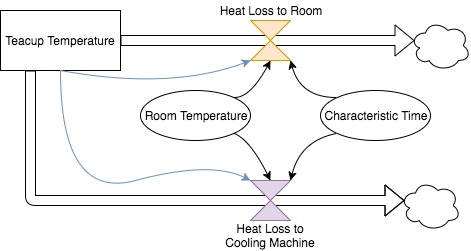
\includegraphics[scale=0.4]{imagenes/Teacup_sd_2}
\caption{Modelo Teacup (versión 2) expresado en SD en formato gráfico}
\label{fig:Teacup_sd_2}
\end{figure}

\begin{figure}[!h]
\centering
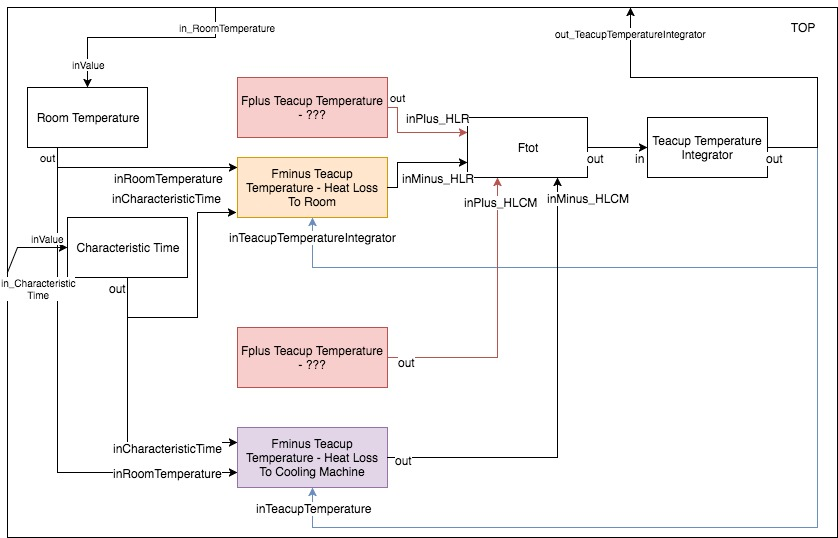
\includegraphics[scale=0.4]{imagenes/Teacup_devs_flattened_2}
\caption{Modelo Teacup (versión 2) expresado en DEVS en formato gráfico}
\label{fig:Teacup_devs_flattened_2}
\end{figure}

Finalmente, pensamos en una forma de modularizar el modelo acoplado tan complejo que quedó tras las conversiones, tanto en la versión original como en la versión 2 del modelo Teacup. Lo que obtuvimos, fue lo que se muestra en las figuras \ref{fig:Teacup_devs} y \ref{fig:Teacup_devs_2}.

Aquí se puede observar que definimos un modelo acoplado por cada \textbf{stock}, que engloba al integrador correspondiente, a la Ftot correspondiente, a los Fminus's correspondientes (outflows que tienen como origen al \textbf{stock} en cuestión), y a los Fplus's correspondientes (inflows que contienen como origen al \textbf{stock} en cuestión). Vale la pena aclarar aquí que dichos, inflows y outflows que operan sobre cada \textbf{stock} corresponden cada uno de ellos a un \textbf{flow} en el modelo expresado en System Dynamics, y es interesante notar que visualmente es muy simple e intuitivo ver cómo se relacionan cada uno de los modelos expresados en SD con su contraparte en DEVS. 

Todos estos serán factores muy importantes a tener en cuenta a la hora de desarrollar la primera versión del traductor, ya que querremos que esta sea lo más general posible, y que sea fácilmente modificable para ser capaz de representar nuevos modelos cada vez más complejos a medida que el proyecto avance.

\begin{figure}[!h]
\centering
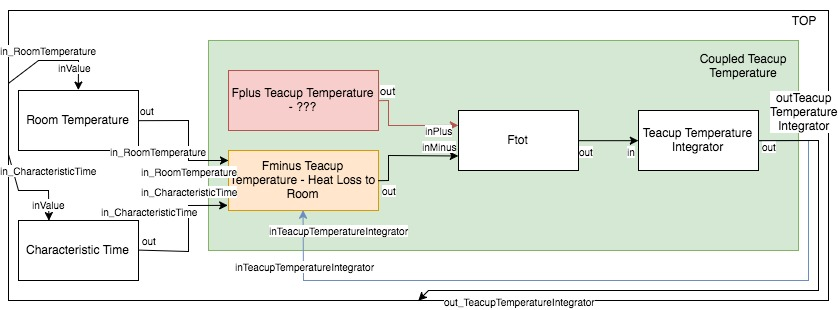
\includegraphics[scale=0.35]{imagenes/Teacup_devs}
\caption{Modelo Teacup expresado en DEVS en formato gráfico utilizando varios niveles de acoplamiento}
\label{fig:Teacup_devs}
\end{figure}
\begin{figure}[!h]
\centering
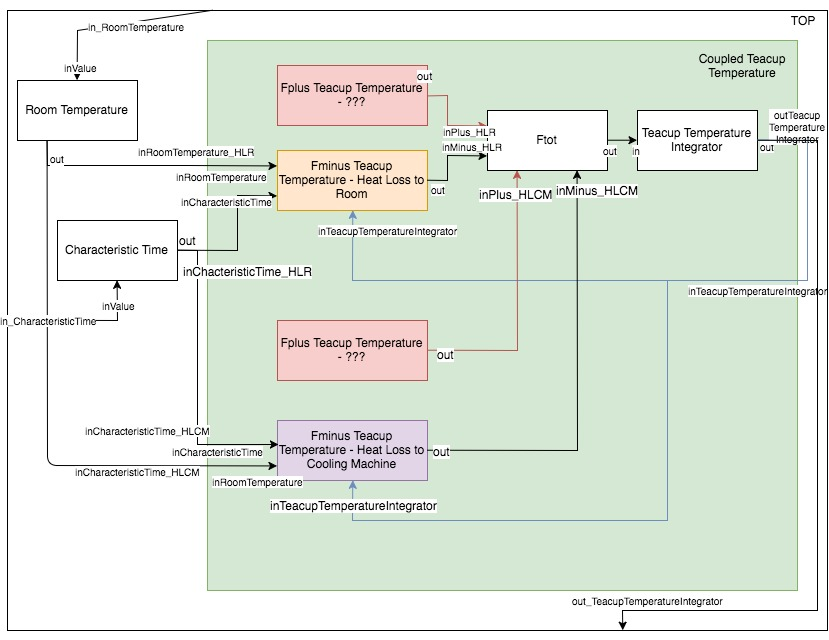
\includegraphics[scale=0.35]{imagenes/Teacup_devs_2}
\caption{Modelo Teacup (versión 2) expresado en DEVS en formato gráfico utilizando varios niveles de acoplamiento}
\label{fig:Teacup_devs_2}
\end{figure}

\subsubsection{Modelo en código}
En esta sección, primeramente mostraremos el modelo .ma que deseamos ser capaces de generar a partir del archivo .devsml generado por nuestro traductor a partir del archivo .xmile del modelo Teacup que ya mencionamos previamente. Por razones de tiempo y para simplificar las cosas en esta primera aproximación al problema, sólo trabajaremos con la versión aplanada del modelo. Es decir, no intentaremos generar varias capas de acoplados, sino un sólo acoplado Top, que contendrá a todos los atómicos que hagan falta.

\begin{figure}[!h]
\centering
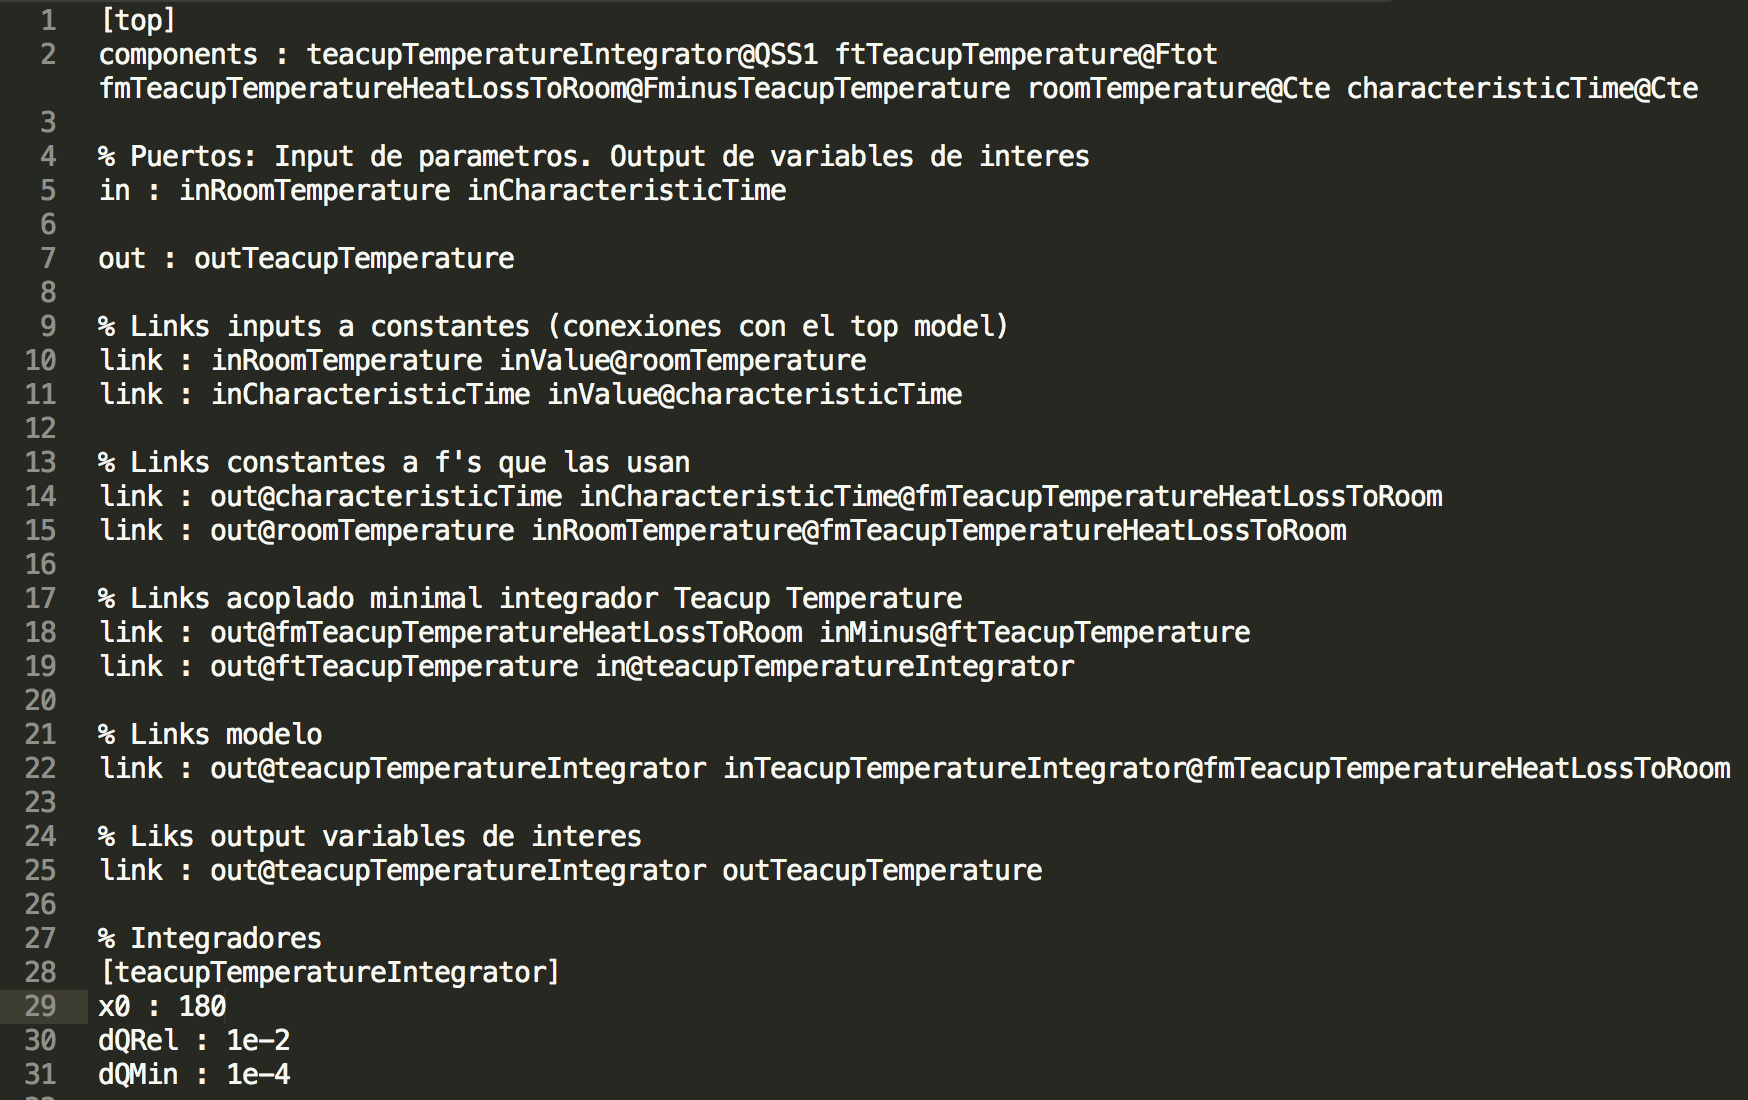
\includegraphics[scale=0.5]{imagenes/teacup_mapeo/Teacup_ma}
\caption{Archivo .ma correspondiente al modelo Teacup para simular el modelo en el simulador CD++}
\label{fig:Teacup_ma}
\end{figure}

Como se puede observar en la figura \ref{fig:Teacup_ma}, el archivo .ma consta de la definición del componente acoplado Top mediante [top], la definición de todos los componentes (modelos atómicos o acoplados, aunque en este ejemplo, como dijimos van a ser todos atómicos) que forman parte del acoplado Top, los puertos de entrada y salida del acoplado (en este caso, la entrada son las variables constantes auxiliares, y la salida es la úncia variable de interés del modelo - la temperatura de la taza -) y los links entre cada uno de los componentes del acoplado.

Compárese la figura \ref{fig:Teacup_devs_flattened} con la figura \ref{fig:Teacup_ma}, y observése el mapeo 1-1 que hay entre cada línea del archivo .ma con el diagrama correspondiente.

Ahora bien, los atómicos utilizados en este modelo, deberán tener un comportamiento. Obviamente, queremos también automatizar la generación de archivos que le den comportamiento a estos atómicos, para que el modelo .ma mostrado más arriba pueda ser ejecutado. Exponemos a continuación las partes más relevantes del código C++ que nuestro traductor genera junto con el .ma para darle el comportamiento deseado a cada atómico.

\begin{figure}[!h]
\centering     %%% not \center
\subfigure[Archvo .h]{\label{fig:Teacup_h}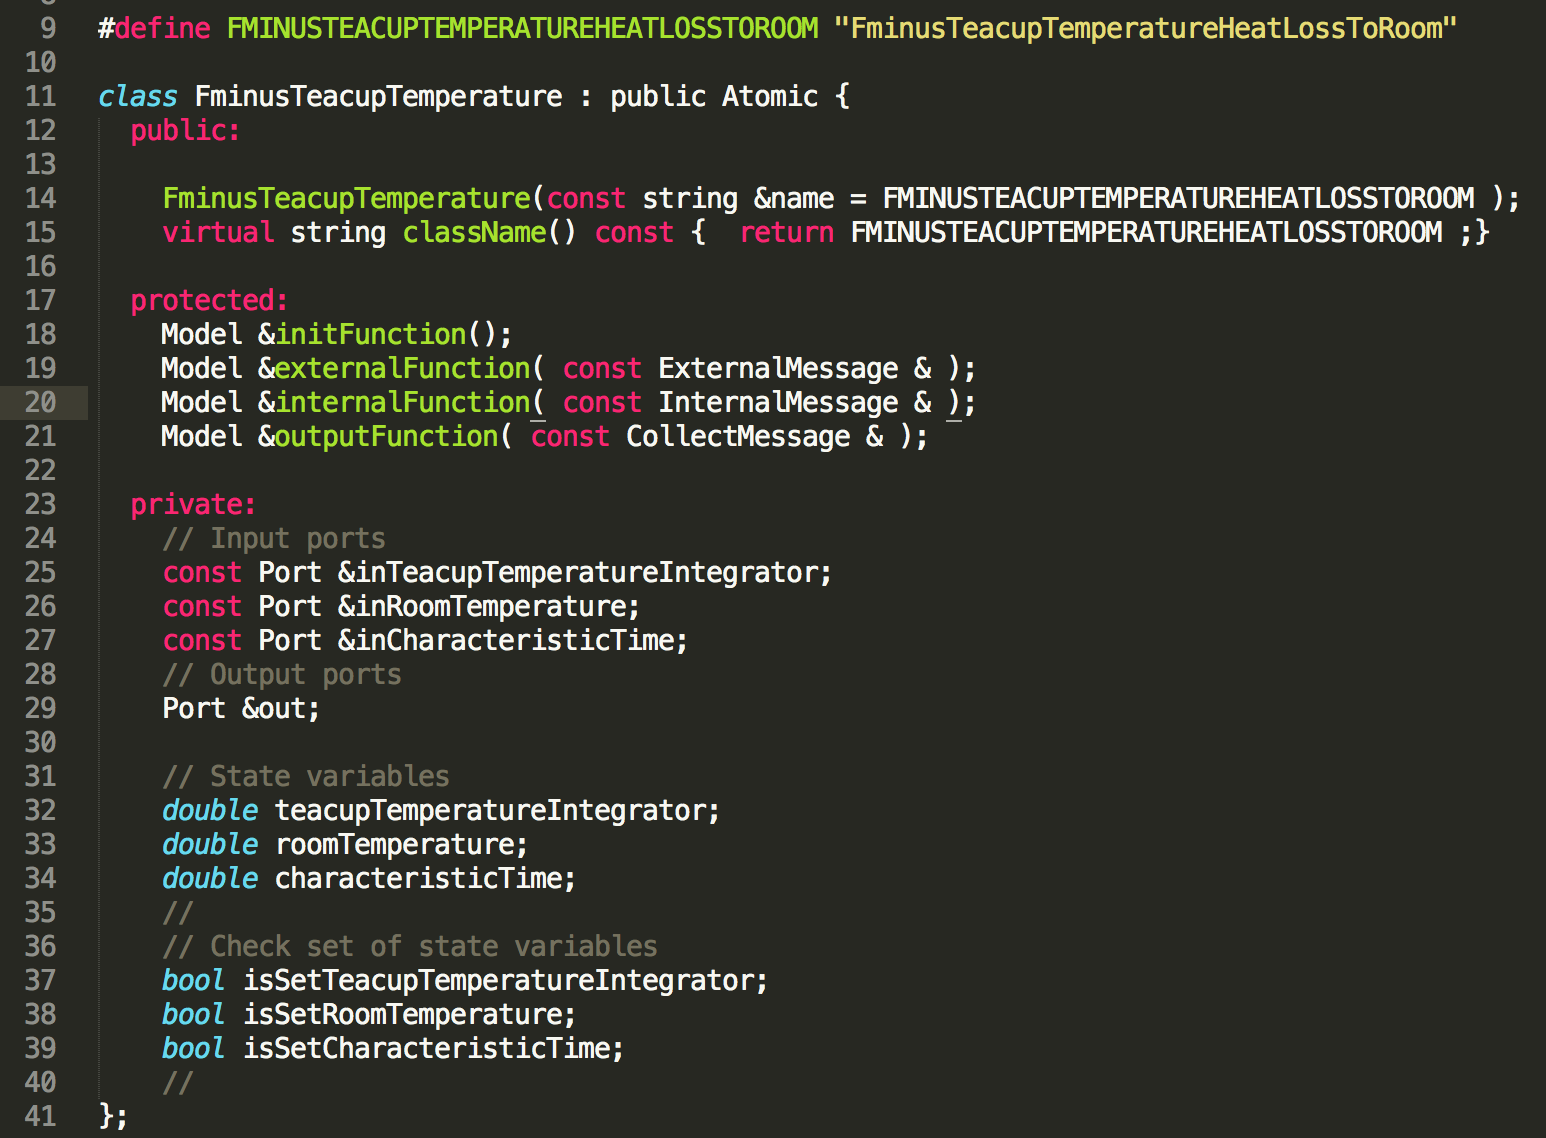
\includegraphics[scale=0.3]{imagenes/teacup_mapeo/Teacup_h}}
\subfigure[Archivo .cpp]{\label{fig:Teacup_hpp}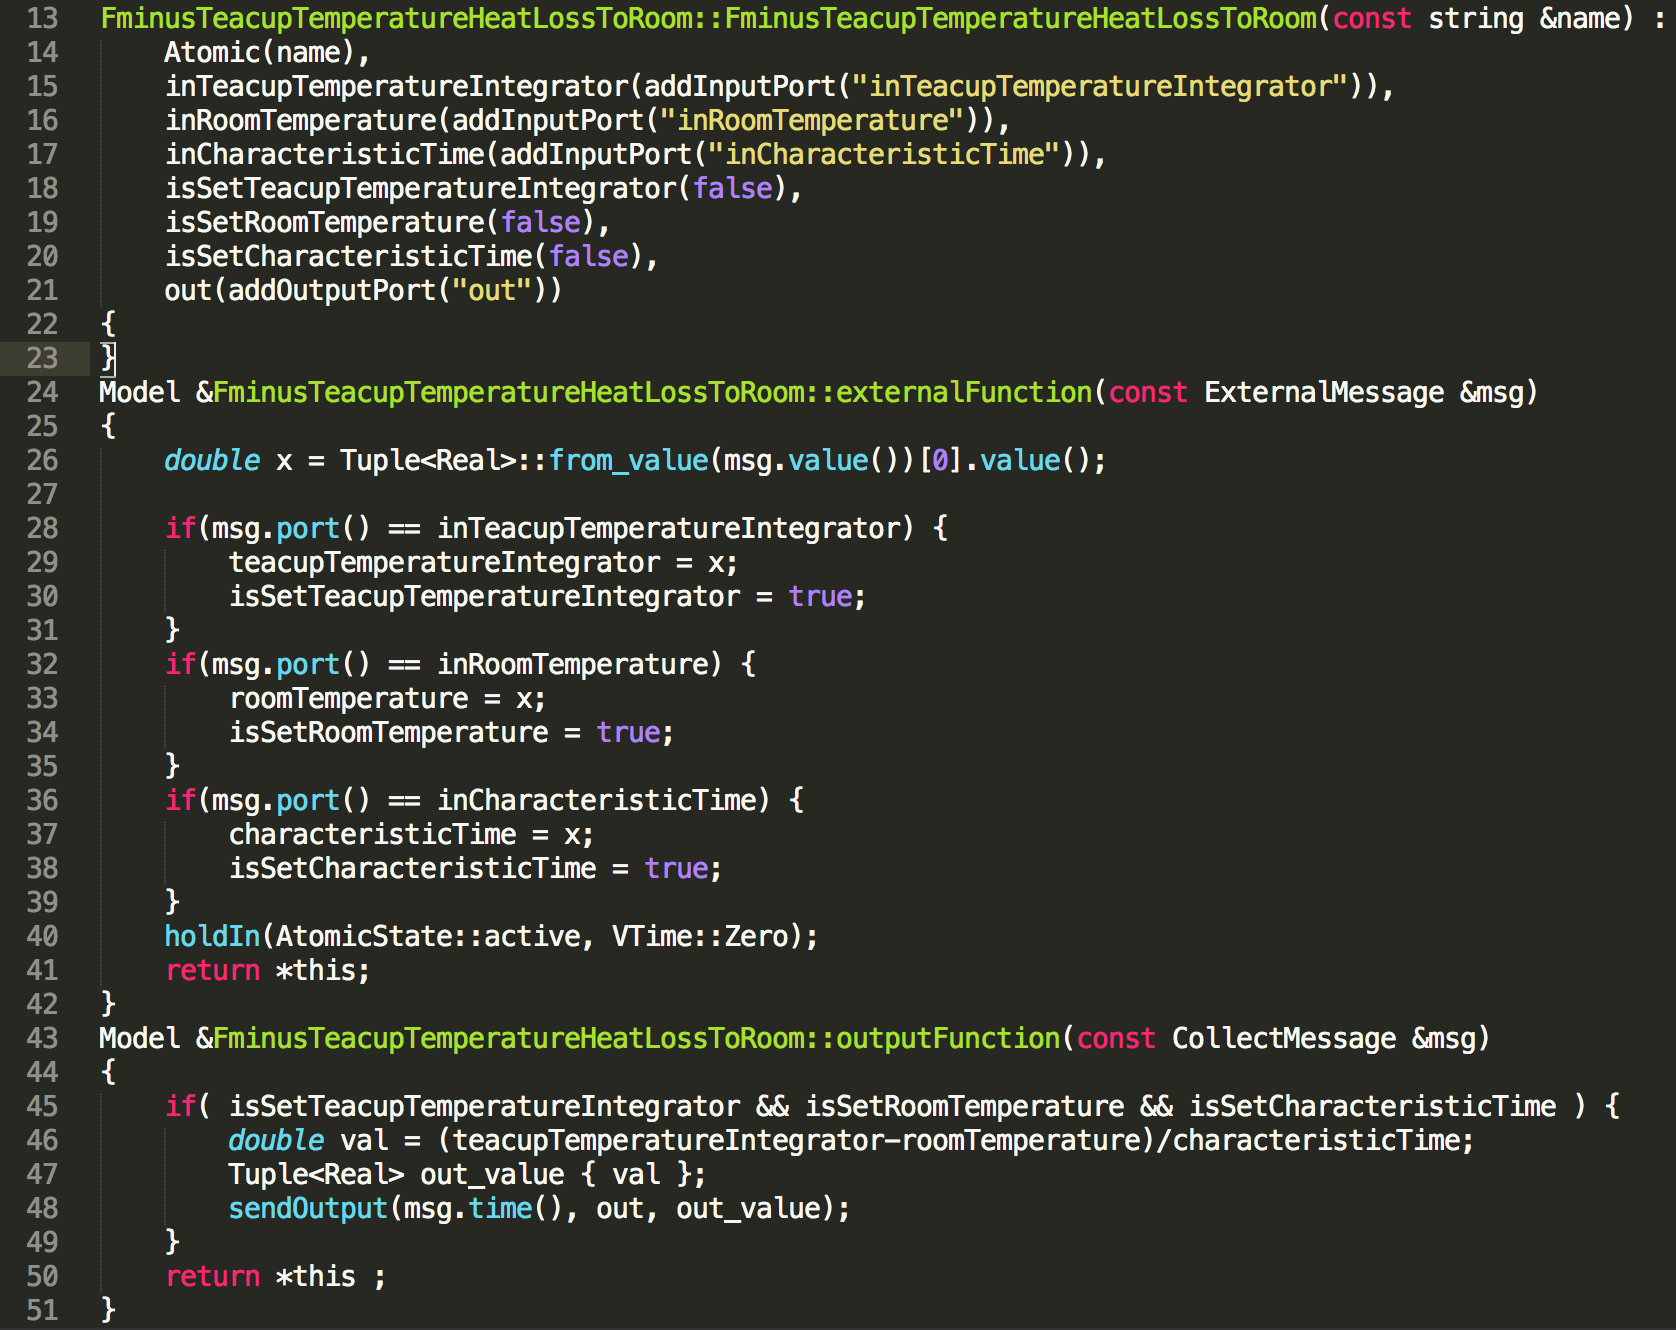
\includegraphics[scale=0.3]{imagenes/teacup_mapeo/Teacup_cpp}}
\caption{Código relevante de los archivos .h y .cpp generados para el atómico FminusTeacupTemperature}
\end{figure}

\begin{figure}[!h]
\centering     %%% not \center
\subfigure[Archvo Ftot.cpp]{\label{fig:Teacup_h}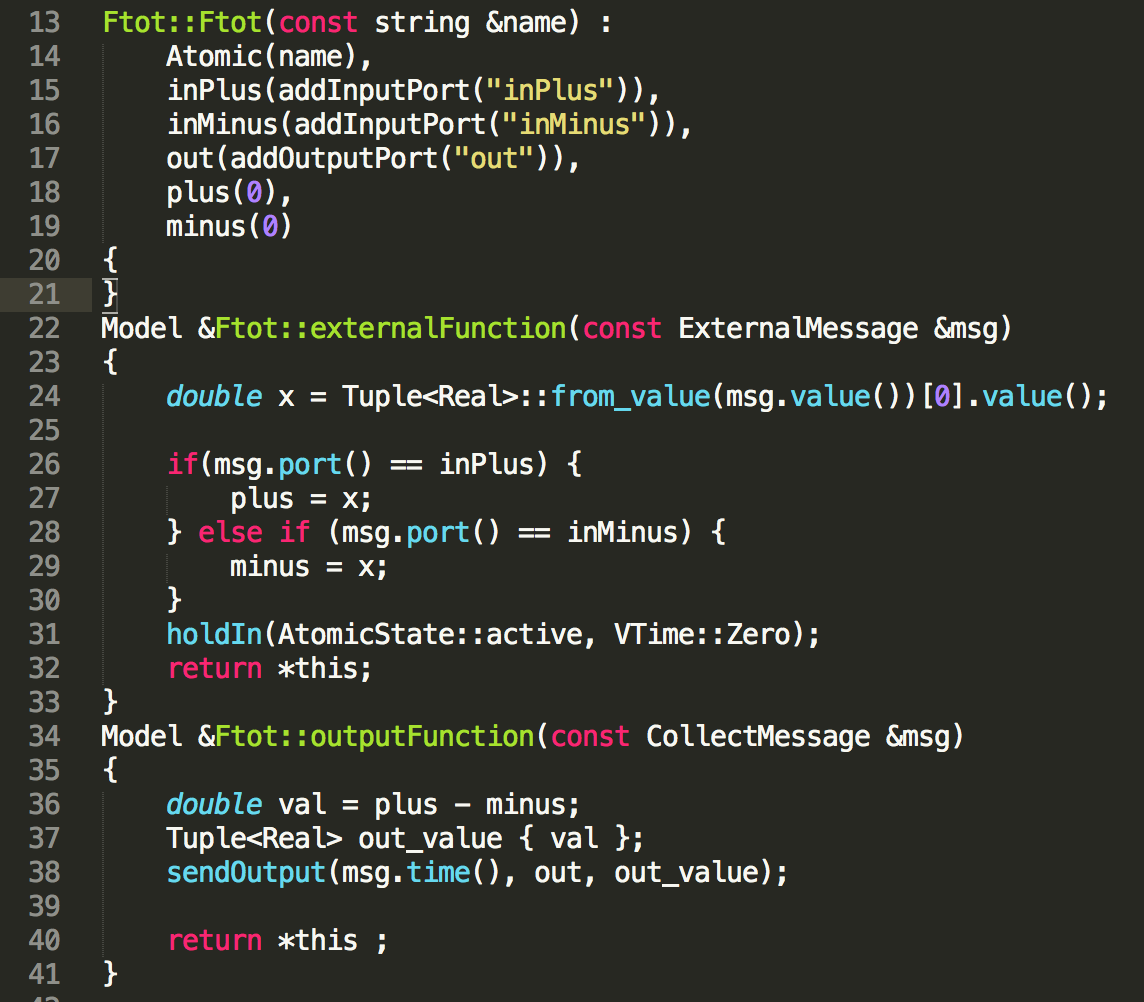
\includegraphics[scale=0.4]{imagenes/gral_mapeo/ftot_cpp}}
\subfigure[Archivo Cte.cpp]{\label{fig:Teacup_hpp}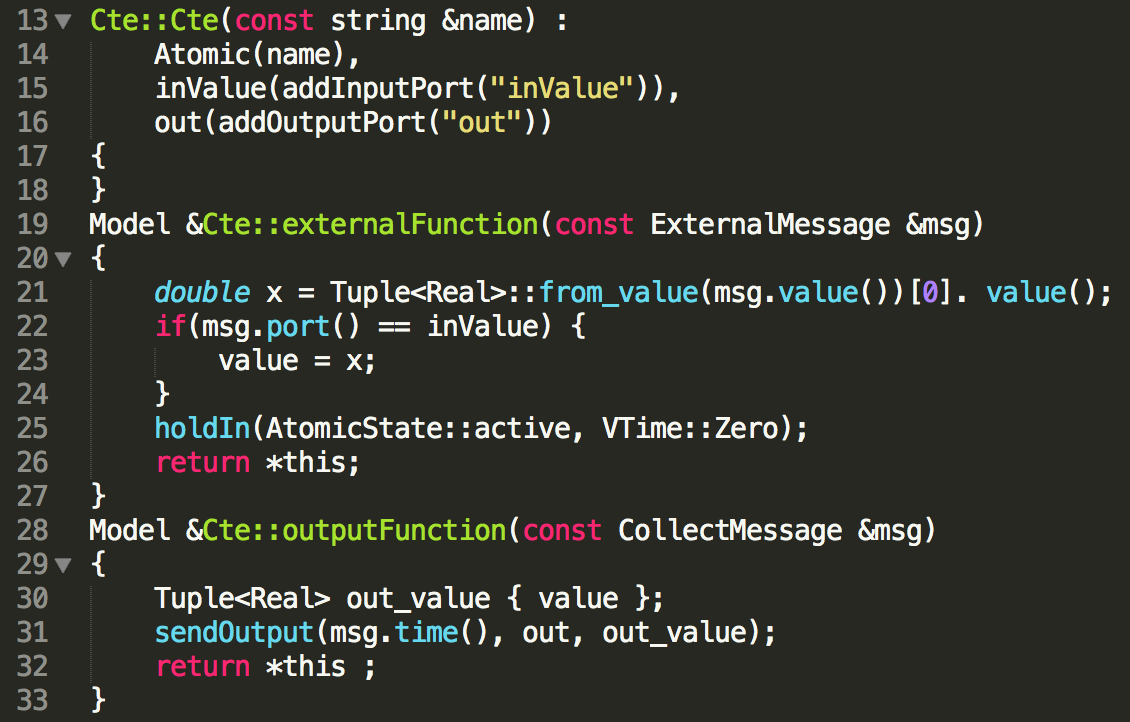
\includegraphics[scale=0.4]{imagenes/gral_mapeo/cte_cpp}}
\caption{Código relevante de los archivos .cpp generados para los atómicos Cte y Ftot}
\end{figure}

\subsubsection{Generación de modelo ejecutable en CD++}
Para poder generar los archivos .ma, .h y .cpp que mencionamos en la sección anterior, previamente debemos generar un archivo .devsml que contenga toda la información necesaria para este fin.

\begin{figure}[!h]
\centering     %%% not \center
\subfigure[Atómicos 1-1 para cada Flow]{\label{fig:Teacup_devsml_components}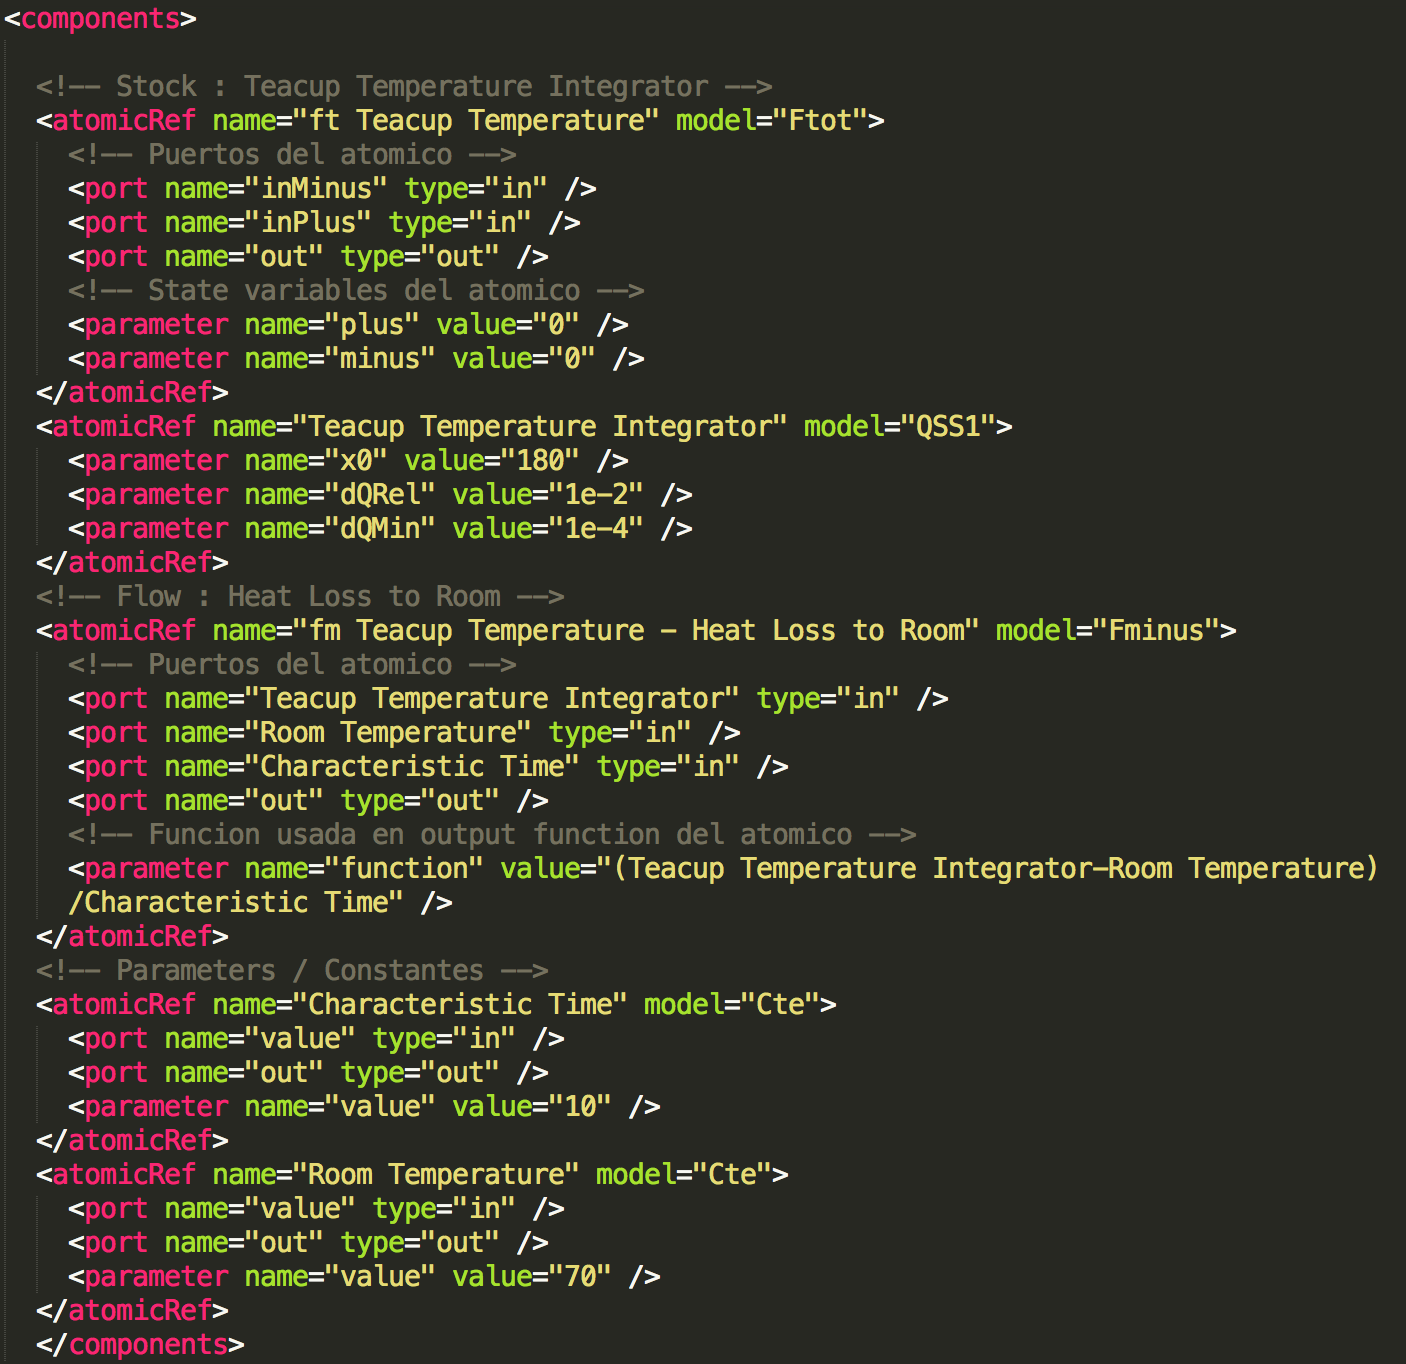
\includegraphics[scale=0.4]{imagenes/teacup_mapeo/Teacup_devsml_components}}
\subfigure[Atómicos 1-1 para cada Stock]{\label{fig:Teacup_devsml_stocks}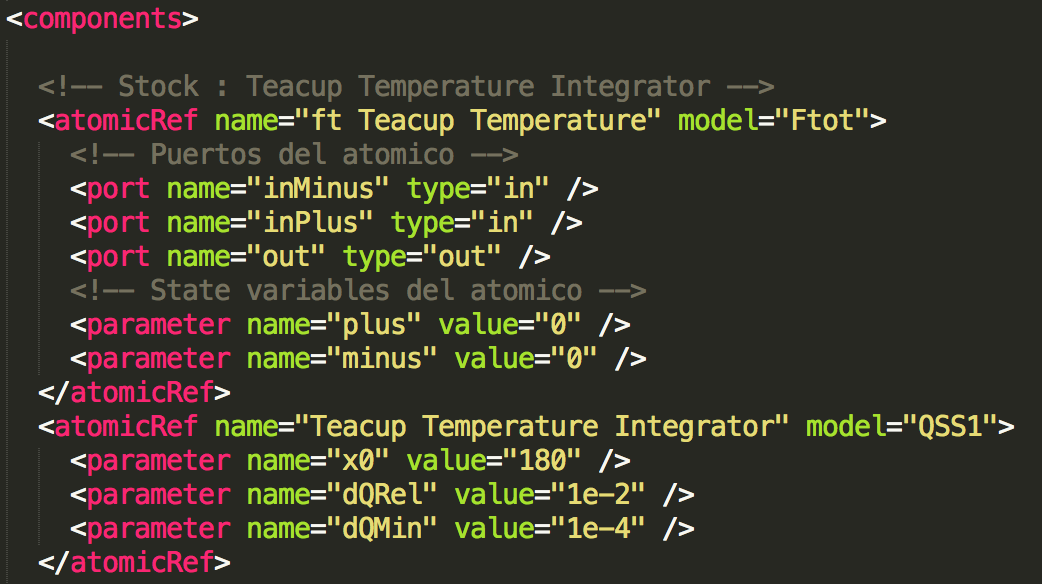
\includegraphics[scale=0.4]{imagenes/teacup_mapeo/Teacup_devsml_stocks}}
\caption{Parte relevante del código .devsml generado por cada Constante, Stock y Flow}
\end{figure}

\begin{figure}[!h]
\centering     %%% not \center
\subfigure[Conexiones internas]{\label{fig:Teacup_devsml_internal_connections}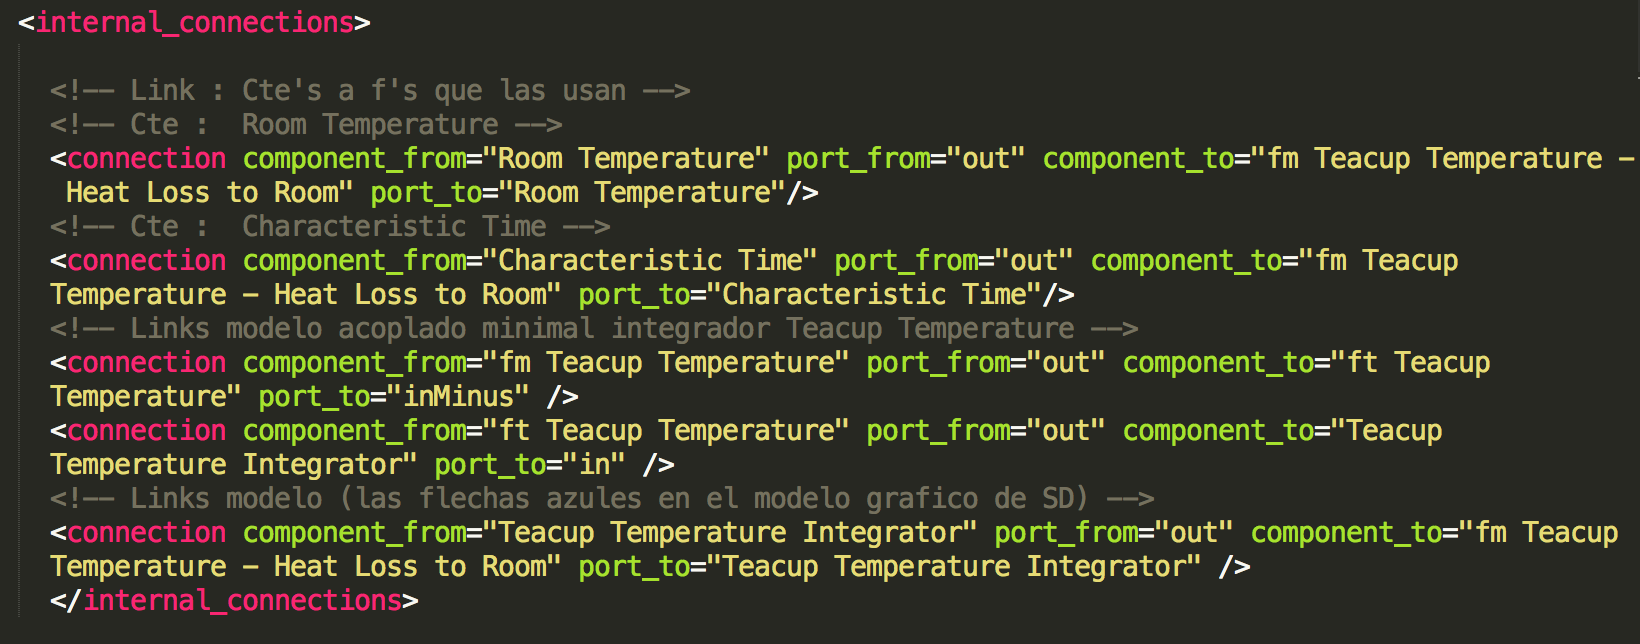
\includegraphics[scale=0.4]{imagenes/teacup_mapeo/Teacup_devsml_internal_connections}}
\subfigure[Conexiones externas]{\label{fig:Teacup_devsml_external_connections}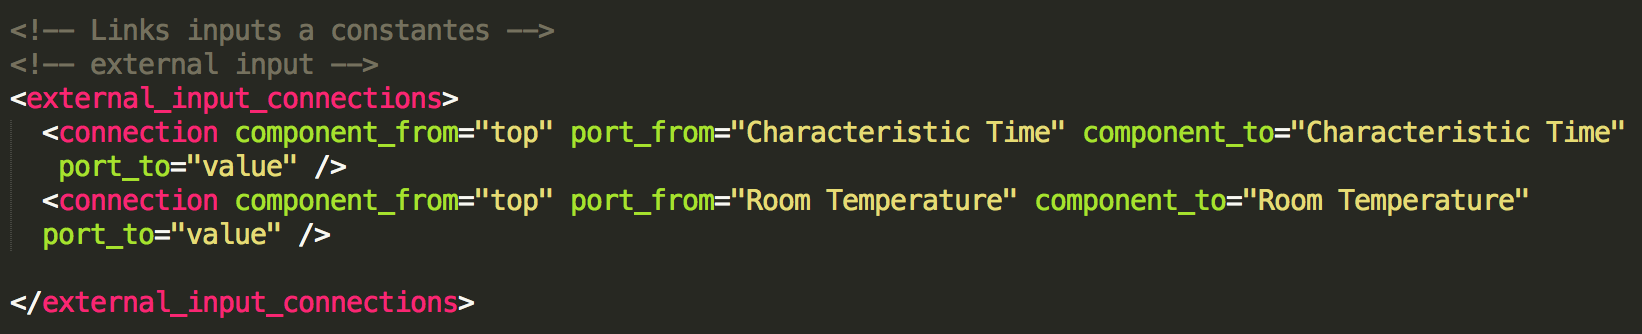
\includegraphics[scale=0.4]{imagenes/teacup_mapeo/Teacup_devsml_external_connections}}
\subfigure[Puertos de entrada/salida del modelo Top]{\label{fig:Teacup_devsml_ports}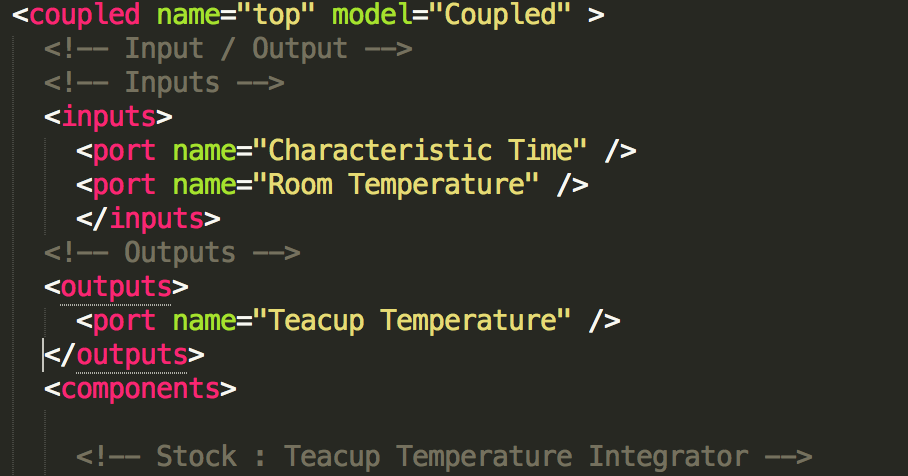
\includegraphics[scale=0.4]{imagenes/teacup_mapeo/Teacup_devsml_ports}}
\caption{Parte relevante del código .devsml generado por cada conexión y para los puertos del modelo Top}
\end{figure}

% TODO
\subsection{Modelo Formal}
Primero mostramos formalmente los modelos atómicos utilizados en el acoplado Top, con la descripción de su comportamiento interno.
\begin{itemize}

\item \textbf{Cte} : $ roomTemperature, characteristicTime \rightarrow \langle X, S, Y, \delta_{int}, \delta_{ext}, \lambda, t_{a} \rangle$ \newline
$ X = \{ inValue \} $ \newline
$ S = \{ value \} $ \newline
$ Y = \{ out \} $ \newline
$ \delta_{int}(\langle value \rangle) = \emptyset $ \newline
$ \delta_{ext} (\langle value \rangle, e, x)= \{ value := x.value \} $ \newline
$ \lambda(\langle value \rangle, out) = value $ \newline
$ t_{a}(s) = \infty $ 

\item \textbf{Fminus} : $ fmTeacupTemperatureHeatLossToRoom \rightarrow \langle X, S, Y, \delta_{int}, \delta_{ext}, \lambda, t_{a} \rangle$ \newline
$ X = \{ inRoomTemperature, inCharacteristicTime, inTeacupTemperatureIntegrator \} $ \newline
$ S = \{ roomTemperature, characteristicTime, teacupTemperatureIntegrator, isSetRoomTemperature, \newline isSetCharacteristicTime, isSetTeacupTemperatureIntegrator \} $ \newline
$ Y = \{ out \} $ \newline
$ \delta_{int}(s) = \emptyset $ \newline
$ \delta_{ext}(s, e, x) = \{
	\\if (x.port = inRoomTemperatureroomTemperature) roomTemperature := x.value; isSetRoomTemperature := true
	\\if (x.port = inCharacteristicTime) characteristicTime := x.value; isSetCharacteristicTime := true
	\\if (x.port = inTeacupTemperatureIntegrator) teacupTemperatureIntegrator = x.value; \\isSetTeacupTemperatureIntegrator := true 
	\} $ \newline
$ \lambda(s, out) = if(todas \ las \ variables \ seteadas) \{ 
\\(teacupTemperatureIntegrator-roomTemperature)/characteristicTime\} \ else \ \emptyset$ \newline
$ t_{a} = \infty $ 

\item \textbf{Ftot} : $ ftTeacupTemperature \rightarrow \langle X, S, Y, \delta_{int}, \delta_{ext}, \lambda, t_{a} \rangle$ \newline
$ X = \{ inMinusHeatLossToRoom \} $ \newline
$ S = \{ plus, minus \} $ \newline
$ Y = \{ out \} $ \newline
$ \delta_{int}(\langle plus, minus \rangle) = \emptyset $ \newline
$ \delta_{ext}(\langle plus, minus \rangle, e, x) = \{ 
	\\if (x.port = inPlus) plus := x.value
	\\if (x.port == inMinusHeatLossToRoom) minus := x.value
	\} $ \newline
$ \lambda(\langle plus, minus \rangle, out) = (plus - minus) $ \newline
$ t_{a} = \infty $ 

\item \textbf{QSS1} : $ teacupTemperatureIntegrator \rightarrow \langle X, S, Y, \delta_{int}, \delta_{ext}, \lambda, t_{a} \rangle$ \newline
$ X = \{ in \} $ \newline
$ S = \{ ? \} $ \newline
$ Y = \{ out \} $ \newline
$ \delta_{int}(s) = \{ ? \} $ \newline
$ \delta_{ext}(s, e, x) = \{ ? \} $ \newline
$ \lambda(s) = ? $ \newline
$ t_{a} = \{ ? \} $ 
\end{itemize}

Ahora que ya tenemos lo atómicos, expresamos el acoplado que utiliza a los atómicos expuestos más arriba:
\begin{itemize}
\item $ Top \rightarrow \langle X, Y, \{ M_{1}, M_{2}, M_{3}, M_{4}, M_{5} \}, C_{xx}, C_{yx}, C_{yy}, Select \rangle$ \newline
$ X = \{ \} $ \newline
$ Y = \{ \} $ \newline
$ M_{1} = roomTemperature $ \newline
$ M_{2} = characteristicTime $ \newline
$ M_{3} = fmTeacupTemperatureHeatLossToRoom$ \newline
$ M_{4} = ftTeacuptTemperature $ \newline
$ M_{5} = teacupTemperatureIntegrator $ \newline
$ C_{xx} = $ \{ \} \newline
$ C_{yx} = \{ (M_{1}.!out, M_{3}.?inRoomTemperture), (M_{2}.!out, M_{3}.?inCharacteristicTime), \\
(M_{5}.!out, M_{3}.?inTecupTemperatureIntegrator), (M_{3}.!out, M_{4}.?inMinusHeatLossToRoom), \\
(M_{4}.!out, M_{5}.?in) \} $ \newline
$ C_{yy} = \{ \} $ \newline
\end{itemize}
% TODO
\subsection{Propuesta de algoritmo traductor}
A continuación, y basándonos en lo aprendido durante la construcción del traductor para el modelo Teacup, detallaremos un algoritmo inicial y muy básico que pensamos debería servir para traducir archivos .xmile a archivos .devsml, a partir de la captura de toda la información relevante contenida en el archivo .xmile.

En esta versión inicial, nos restringimos a traducir a modelos DEVS aplanados solamente. De esta manera, se simplifican algunos detalles de la implementación del traductor. Además de estos, nos restringimos a archivos .xmile que también estén aplanados. Es decir, no lidiamos con la presencia de diferentes módulos con modelos internos, y la interacción de los modelos internos a través de los módulos en lugar de directamente. De este problema nos encargaremos más adelante, cuando estudiemos el modelo Lotka-Volterra.

Para este fin, dividiremos la explicación del algoritmo en partes, para explicar las figuras \ref{fig:Teacup_devsml_components}, \ref{fig:Teacup_devsml_stocks}, \ref{fig:Teacup_devsml_internal_connections}, \ref{fig:Teacup_devsml_external_connections} y \ref{fig:Teacup_devsml_ports}, explicando como cada una de estas se corresponde con las líneas del archivo .ma expuesto en la figura \ref{fig:Teacup_ma}.

\subsubsection{Traducción de \textbf{Stocks}}
\subsubsection{Traducción de \textbf{Flows}}
\subsubsection{Generación de puertos es E/S del modelo DEVS}
\subsubsection{Generación de conexiones internas del modelo DEVS}
\subsubsection{Generación de conexiones externas del modelo DEVS}

% TODO
\subsection{Modelo SIR}
\subsubsection{Modelo gráfico}
En la figura \ref{fig:SIR_devs_flattened} se observa en color azul los atómicos Fplus y Fminus asociados al flujo \textit{Succumbing}, mientras que en naranja se observan los atómicos Fplus y Fminus asociados al flujo \textit{Recovering}. En violeta se pueden ver las conexiones que representan de qué manera los diferentes atómicos correspondientes a cada uno de los flujos utilizan para realizar sus cálculos internos el output de \textit{InfectedIntegrator}, correspondiéndose cada una de estas flechas con una de las flechas del modelo gráfico mostrado en la figura \ref{fig:SIR_sd}. Como ya explicamos anteriormente, en este ejemplo sólo trabajaremos con la versión aplanada del modelo DEVS, para simplificar levemente el problema de traducción. 

Nuevamente, dejamos en rojo los atómicos que no tienen cabida en el modelo, pero que igualmente exponemos, para dejar explícito que esos atómicos podrían estar si hubiera un inflow/outflow que se les corresponda, pero que en este ejemplo no lo están.
\begin{figure}[!h]
\centering
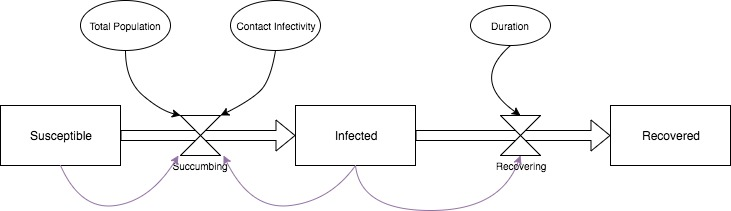
\includegraphics[scale=0.5]{imagenes/SIR_sd.jpg}
\caption{Modelo SIR expresado en System Dynamics en formato gráfico}
\label{fig:SIR_sd}
\end{figure}
\begin{figure}[!h]
\centering
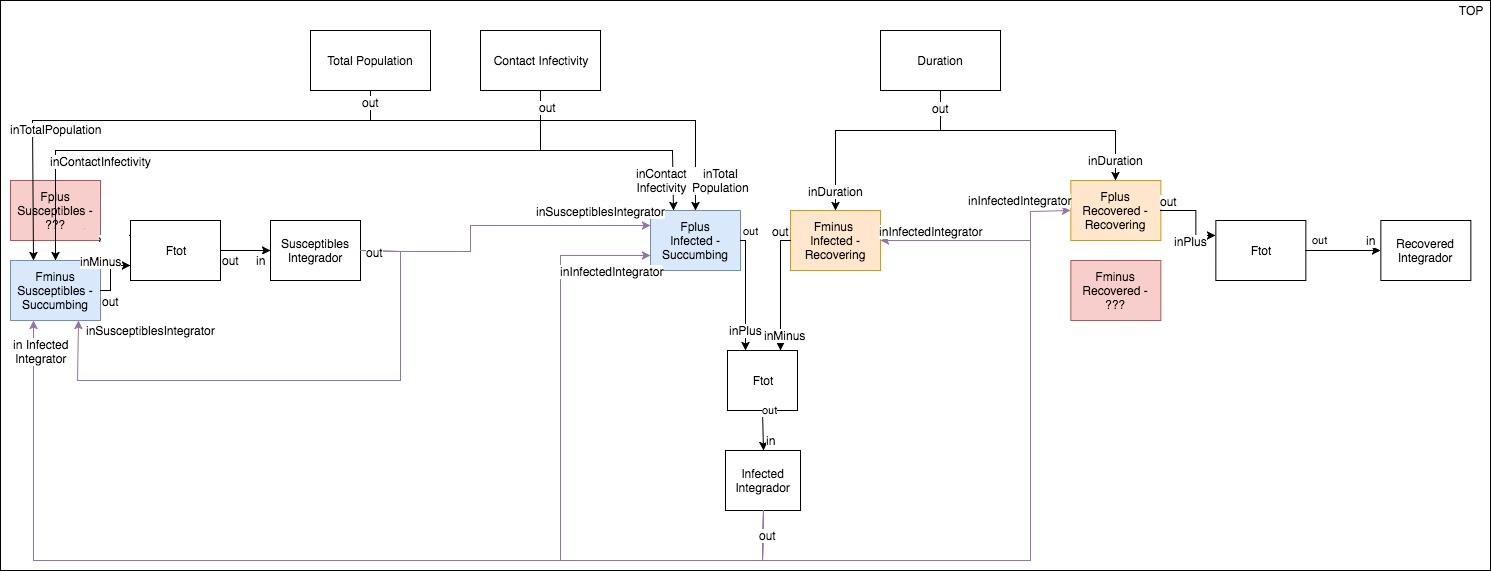
\includegraphics[scale=0.3]{imagenes/SIR_devs_flattened.jpg}
\caption{Modelo SIR expresado en DEVS en formato gráfico}
\label{fig:SIR_devs_flattened}
\end{figure}
\begin{figure}[!h]
\centering
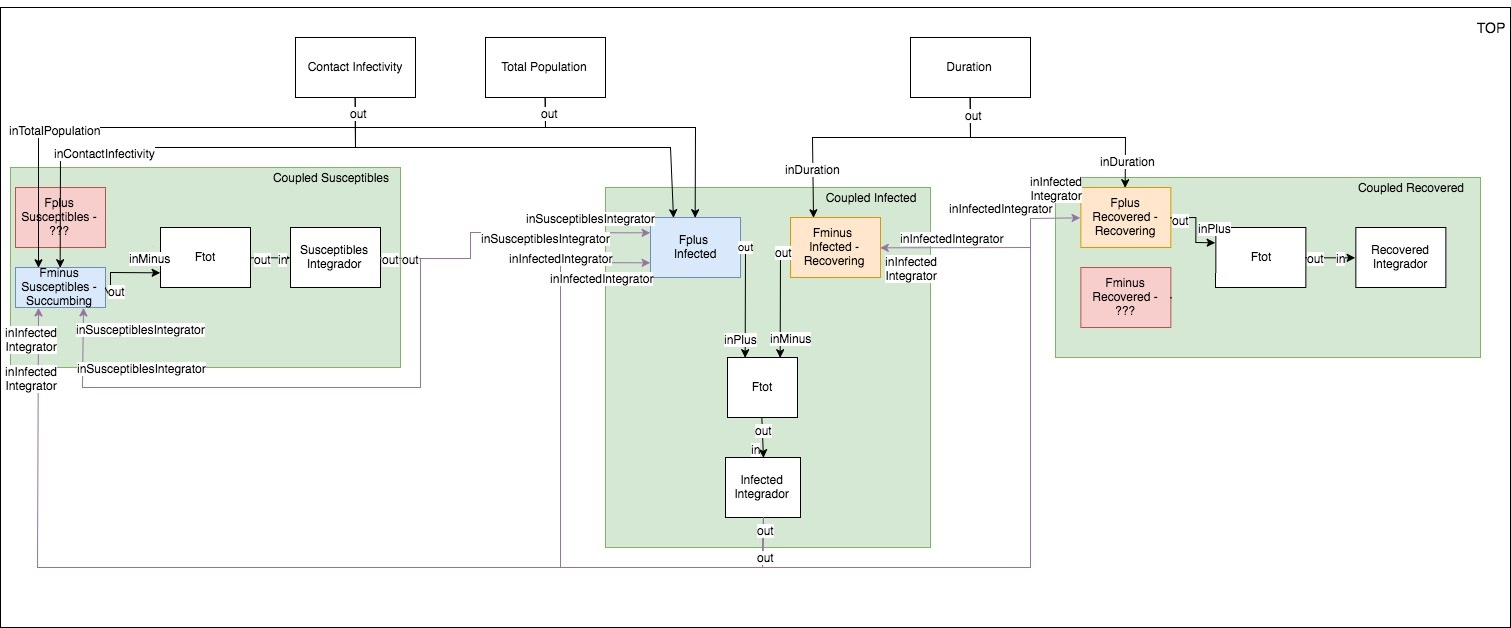
\includegraphics[scale=0.3]{imagenes/SIR_devs.jpg}
\caption{Modelo SIR expresado en DEVS en formato gráfico con varios niveles de acoplamiento}
\label{fig:SIR_devs}
\end{figure}
% TODO
\subsubsection{Modelo formal}
A continuación, exponemos formalmente los modelos atómicos utilizados en el acoplado Top, con la descripción de su comportamiento interno.
\begin{itemize}
\item \textbf{Cte} : $ totalPopulation \rightarrow \langle X, S, Y, \delta_{int}, \delta_{ext}, \lambda, t_{a} \rangle$
\item \textbf{Cte} : $ contactInfectivity \rightarrow \langle X, S, Y, \delta_{int}, \delta_{ext}, \lambda, t_{a} \rangle$
\item \textbf{Cte} : $ duration \rightarrow \langle X, S, Y, \delta_{int}, \delta_{ext}, \lambda, t_{a} \rangle$
\item \textbf{Fminus} : $ fmSusceptiblesSuccumbing \rightarrow \langle X, S, Y, \delta_{int}, \delta_{ext}, \lambda, t_{a} \rangle$
\item \textbf{Ftot} : $ ftSusceptibles \rightarrow \langle X, S, Y, \delta_{int}, \delta_{ext}, \lambda, t_{a} \rangle$
\item \textbf{QSS1} : $ susceptiblesIntegrator \rightarrow \langle X, S, Y, \delta_{int}, \delta_{ext}, \lambda, t_{a} \rangle$
\item \textbf{Fplus} : $ fpInfectedSuccumbing \rightarrow \langle X, S, Y, \delta_{int}, \delta_{ext}, \lambda, t_{a} \rangle$
\item \textbf{Fminus} : $ fmInfectedRecovering \rightarrow \langle X, S, Y, \delta_{int}, \delta_{ext}, \lambda, t_{a} \rangle$
\item \textbf{Ftot} : $ ftInfected \rightarrow \langle X, S, Y, \delta_{int}, \delta_{ext}, \lambda, t_{a} \rangle$
\item \textbf{QSS1} : $ infectedIntegrator \rightarrow \langle X, S, Y, \delta_{int}, \delta_{ext}, \lambda, t_{a} \rangle$
\item \textbf{Fplus} : $ fpRecoveredRecovering \rightarrow \langle X, S, Y, \delta_{int}, \delta_{ext}, \lambda, t_{a} \rangle$
\item \textbf{Ftot} : $ ftRecovered \rightarrow \langle X, S, Y, \delta_{int}, \delta_{ext}, \lambda, t_{a} \rangle$
\item \textbf{QSS1} : $ recoveredIntegrator \rightarrow \langle X, S, Y, \delta_{int}, \delta_{ext}, \lambda, t_{a} \rangle$
\end{itemize}

\subsubsection{Generación de modelo ejecutable en CD++}


\subsection{Modelo Lotka-Volterra}
